\documentclass{vldb}

\usepackage{balance}
\usepackage{url} 
\usepackage{times}
%For math symbols like number classes
\usepackage{amsfonts}
\usepackage{amssymb}
%\usepackage{amsthm}
%\usepackage{floatflt}
\usepackage{wrapfig}
\usepackage{multirow}
\usepackage{color}

\usepackage[T1]{fontenc}
\usepackage{hyperref}
\usepackage{amsmath}
\usepackage{acronym}
\interdisplaylinepenalty=2500
\usepackage{xspace} % mellemrum efter forkortelser fra acronym package.
\usepackage{longtable}
\usepackage{graphicx}
\usepackage{graphics}
\usepackage{slashbox}
\usepackage{pstricks}

% \usepackage[cmex10]{amsmath}
% \usepackage[pdftex]{graphicx}
% \usepackage[pdftex]{graphics}


% \usepackage[boxed,linesnumbered,vlined,slide]{algorithm2eCustom}
\usepackage[boxed,linesnumbered,vlined,ruled]{algorithm2eCustom}

\usepackage{cite}


% correct bad hyphenation here
\hyphenation{op-tical net-works semi-conduc-tor}


\begin{document}
\newcommand{\ffh}[1]{\textbf{TODO: \textit{#1}}} 

\newcommand{\mdns}{\ac{MD}}
\newcommand{\md}{\mdns \xspace}
\newcommand{\mdsns}{{\mdns}'s}
\newcommand{\mds}{\mdsns \xspace}

\newcommand{\ls}{\lsns \xspace}
\newcommand{\lsns}{LS}
\newcommand{\lss}{\lssns \xspace}
\newcommand{\lssns}{LSs}

\newcommand{\spathns}{\ac{SP}}
\newcommand{\spath}{\spathns \xspace}
\newcommand{\spathsns}{{\spathns}s}
\newcommand{\spaths}{\spathsns \xspace}

\newcommand{\oscns}{\ac{OSC}}
\newcommand{\osc}{\oscns \xspace}

\newcommand{\lruns}{\ac{LRU}}
\newcommand{\lru}{\lruns \xspace}
\newcommand{\lrusns}{{\lruns}s}
\newcommand{\lrus}{\lrusns \xspace}

\newcommand{\fifons}{\ac{FIFO}}
\newcommand{\fifo}{\fifons \xspace}

\newcommand{\spsns}{\ac{SPS}}
\newcommand{\sps}{\spsns \xspace}

\newcommand{\salgons}{$\mathsf{PScache}$}
\newcommand{\salgo}{\salgons \xspace}

\newcommand{\poins}{\ac{POI}}
\newcommand{\poi}{\poins \xspace}
\newcommand{\poisns}{{\poins}'s}
\newcommand{\pois}{\poisns \xspace}

\newcommand{\naive}{\naivens \xspace}
\newcommand{\fair}{\fairns \xspace}
\newcommand{\naivens}{\textbf{Naive}}
\newcommand{\fairns}{\textbf{Fair}}

\newcommand{\zebox}[1]{$|\underline{\overline{#1}}|$}

\newcommand{\lpar}{(}
\newcommand{\rpar}{)}

\SetKwBlockLRS{JRBegin}
\newcommand{\funcc}[3]{\emph{\textbf{#1}}\ensuremath{\lpar #2 \rpar} \JRBegin{#3}}
%\newcommand{\func}[2]{\emph{\textbf{#1}}\ensuremath{\lpar #2 \rpar} \\}


%To change extension of algorithm2e use \algoext{A}, \algoext{B}, \Algoext{}
\newcommand{\algoext}[1]{\renewcommand{\thealgoext}{#1}}
\newtheorem{thm}{Theorem}[section]
\newtheorem{cor}[thm]{Corollary}
\newtheorem{lemma}[thm]{Lemma}

%proof and definitions will not get numbers, meant to be used with lemma/corollary/theorem
%like definition ... lemma (with numbering to reference) ... proof
\newenvironment{definition}[1][Definition]{\begin{trivlist}
\item[\hskip \labelsep {\bfseries #1}]}{\end{trivlist}}



\SetKwBlockLRS{JRBegin}
\pagestyle{plain}

\title{Shortest Path Cache \\
%\titlenote{for use with vldb.cls, (no clue what that means..)}\\ 
{\textit{\small \today}}
}

\numberofauthors{2} 
\author{
% 1st. author
\alignauthor
Jeppe Rishede Thomsen \\%\titlenote{some author note, 1}\\
       \affaddr{Department of Computing}\\
       \affaddr{Hong Kong Polytechnic University}\\
       \affaddr{Kowloon, Hong Kong}\\
       \email{csjrthomsen@comp.polyu.edu.hk}
% 2nd. author
\alignauthor
Man Lung Yiu \\
       \affaddr{Department of Computing}\\
       \affaddr{Hong Kong Polytechnic University}\\
       \affaddr{Kowloon, Hong Kong}\\
       \email{csmlyiu@comp.polyu.edu.hk}
% % 3rd. author
% \alignauthor Lars Th{\Large{\sf{\o}}}rv{$\ddot{\mbox{a}}$}ld\titlenote{This author is the
% one who did all the really hard work.}\\
%        \affaddr{The Th{\large{\sf{\o}}}rv{$\ddot{\mbox{a}}$}ld Group}\\
%        \affaddr{1 Th{\large{\sf{\o}}}rv{$\ddot{\mbox{a}}$}ld Circle}\\
%        \affaddr{Hekla, Iceland}\\
%        \email{larst@affiliation.org}
}


\maketitle

%\acrodef{acronym}{definition}
\acrodef{MD}{Mobile Device}

\acrodef{CFG}{Context-Free Grammar}

\acrodef{CNF}{Chomsky Normal Form}

\acrodef{BNF}{Backus-Naur Form}

\acrodef{EBNF}{Extended Backus-Naur Form}

\acrodef{AST}{Abstract Syntax Tree}

\acrodef{LALR}{Look-Ahead Left-to-Right}

\acrodef{CLR}{Common Language Runtime}

\acrodef{CTS}{Common Type System}

\acrodef{IDE}{Integrated Development Enviroment}

\acrodef{LoC}{Lines of Code}

\acrodef{GUI}{Graphical User Interface}

\acrodef{UI}{User Interface}

\acrodef{AS} {Always Sensitive} 

\acrodef{ASTI} {Always Sensitive with time interval} 

\acrodef{ASST} {Often Sensitive at specific time}
	
\acrodef{RS} {Rarely sensitive}

\acrodef{PSR} {Potential Sensitive Region}

\acrodef{RT} {Road Type}

\acrodef{SSSP} {Single Source Shortest Path}

\acrodef{SP} {Shortest Path}

\acrodef{OSC} {Optimal Substructure Cache}

\acrodef{LRU} {Least Recently Used}

\acrodef{FIFO} {First In, First Out}

\acrodef{SPS} {\spath subpath Sharing}
\begin{abstract}
% All the papers either solve the problem of a more efficient cache in a specific domain, or use the network domain,  which are both relevant, but not really useful when looking at shortest path caching.
% 
% The papers show some interesting ways to use cache, but ultimately their approaches are very domain or query specific so their approaches to caching and cache replacement/invalidation can not be applied directly.


abstract...

Lorem ipsum dolor sit amet, consectetur adipiscing elit. Nunc luctus mattis pretium. Mauris egestas risus non lectus dapibus condimentum. Vestibulum at lacus sit amet elit rutrum venenatis sit amet sed turpis. Nam ullamcorper, urna aliquet venenatis tempor, dolor enim egestas neque, ac feugiat felis neque et libero. Vivamus in augue urna. Integer euismod interdum felis, a porta quam posuere at. Duis molestie leo ullamcorper mauris sodales porta. Praesent cursus, tortor a iaculis blandit, mauris tellus suscipit nibh, in condimentum elit eros nec mauris. In hac habitasse platea dictumst.

Phasellus eget tortor eget diam dignissim pretium nec ut nibh. Morbi bibendum nibh et eros tristique rhoncus. Suspendisse dolor erat, lacinia ut ullamcorper vitae, dictum nec dolor. Etiam egestas tempus fermentum. Donec commodo feugiat lorem. Donec facilisis pharetra leo, sit amet cursus turpis convallis eu. Sed fermentum sapien quam, quis porttitor est.
\end{abstract}

\section{Multi-weight} \label{sec:intro}


\begin{table}
\begin{tabular*}{\columnwidth}{|l|p{0.76\columnwidth}|}
\hline
\bf Symbol		& \bf Meaning \\\hline
$G\mathbf{(V,E)}$ 	& A graph with node set $V$ and edge set $E$ \\\hline 
$v_i$			& A node in $V$ \\\hline 
$(v_i,v_j)$		& An edge in $E$ \\\hline 
$\omega_k(v_i,v_j)$	& The edge weight of $(v_i,v_j)$ using weight category $\varsigma_k \in \mathcal{W}$ \\\hline
$\mathcal{W}$		& Set of possible weight categories $\mathcal{W}$, where $\varsigma_k$ denotes the category $k$ \\\hline

$Q_{s,t,w}$		& \spath query from node $v_s$ to node $v_t$, using weight $w$\\\hline
$P_{s,t,w}$		& The \spath result of $Q_{s,t,w}$ \\\hline
$|P_{s,t,w}|$		& The size of $P_{s,t,w}$ (in number of nodes) \\\hline
$E_{s,t,w}$		& The expense of executing query $Q_{s,t,w}$ \\\hline
$\chi_{s,t,w}$		& The frequency of a \spath with weight type w \\\hline
$\Psi$ 			& The Cache \\\hline
$\mathfrak{U}^w(P_{s,t,w})$& The set of all subpaths in $P_{s,t,w}$ \\\hline
$\mathfrak{U}^w(\Psi)$	& The set of all subpaths of paths in $\Psi$ \\\hline
$\gamma^w(\Psi)$		& The total benefit of the content in the cache \\\hline

$d_{s,t,w}$		& The \spath distance of a path $P_{s,t,w}$ \\\hline
$\mathcal{QL}^w$		& Query log of search queries \\\hline
\end{tabular*}
\caption{Table of Symbols \textbf{MW}}
\label{tab:symbols}
\end{table}

% 
% 
% \begin{algorithm}[bht]
% \dontprintsemicolon
% \SetVline
% 
% \SetKwInOut{Input}{input}\SetKwInOut{Output}{output}\SetKw{Return}{return}
% 
% \Input{
% 
% 	$(q,R)$: A Range query\;
% 	$\mathcal{O}$: A set of POI \;
% }
% 
% \Output{
% 
% 	A set \poi $\in \mathcal{O}$ \;
% }
% 
% \funcc{Fair}{(q,R), \mathcal{O}}
% {
%     \ForEach{$o_i \in \mathcal{O} : \mathfrak{d}_{q,o_i} \leq R$}
%     {
%       $candidate_{\mathcal{O}} \leftarrow o_i$ \;
%     }
%     result $\leftarrow$ \naivens((q,R), $candidate_{\mathcal{O}}$) \;
% 
%     \Return{result} \;
% }
% 
% \caption{Fair Algorithm}
% \label{alg:fair}
% \end{algorithm}


In multi-weight road networks\cite{icdeMouratidisLY10} a shortest path query may be submitted to a service provider based on different shortest path metrics or categories. A category could be the fastest route, the fewest number of edges to traverse, or of cause the actual shortest distance. These kind of queries require the \spath service provider to have several weights defined for each edge, a fair assumption on most service providers (TODO: CITE).
Such queries present a challenge to effectively cache, as the same \spath $P_{s,t,w}$ may not be valid for all weights/metrics $w$.
Two queries with identical start- and end-point can return two different \spathsns, depending on what weight category is issued with the query. Figure \ref{fig:map1} shows a map with two weight categories on each edge, $w_1,w_2$. The two queries $Q_{1,6,w_1}$ \& $Q_{1,6,w_2}$ are identical, except for the weight category. $\psi_1$ and $\psi_2$ in table \ref{tab:expsi} show the \spath result of the two queries in column "cache item". It is clear that the result of the two queries are very different because of the difference in weight category used for each result.




\begin{definition}
Let $G(V, E)$ be a graph with a set $V$ of nodes and a set $E$ of edges.
Each node $v_i \in V$ models a road junction. Each edge $(v_i, v_j) \in
E$ models a road segment. The weight or 'length' of an edge is denoted as $W(v_i, v_j, w)$, where $w \in \mathcal{W}$ is the weight type (length, travel time, scenic value, ect.).
\end{definition}



\begin{definition}{Multi-weight Search}\\
A Multi-weight Search query, denoted by $Q_{s,t,w}$ consist of a source and target vertex $s$ and $t$, plus a category $w \in \mathcal{W}$ 
The result of $Q_{s,t,w}$, denoted $P_{s,t,w}$, is a collection of connected vertices $v_s,\dotsc,v_t$ such that they form a \spath on graph $G\mathbf{(V,E)}$ using category $w \in \mathcal{W}$.
\end{definition}


Using the map1 (fig. \ref{fig:map1}) a multi-weight search query, $Q_{1,2,w}$, can be executed for two different weights, $w_1$ or $w_2$, possibly resulting in two different paths for the same start-/end-nodes, depending on the weight chosen. Table \ref{tab:expsi} shows the \spath $\psi_1$ and $\psi_2$ resulting from the same start-/end-node, but using different weights ($w_1, w_2$).


\begin{figure}[hbt]
  \center
        \includegraphics[width=0.4\textwidth]{figures/map1}
        \caption{Map1. Has a set of two weights on each edge, $w_1,w_2$.}
  \label{fig:map1}
\end{figure}

\begin{table}
\begin{tabular}{l|l|l}\hline
$\psi$		& Cache item 			& Category \\\hline  \hline
$\psi_1:$	& $\{v_1,v_3,v_4,v_5,v_6\}$ 	& ($w_1$)\\\hline
$\psi_2:$	& $\{v_1,v_3,v_6\}$ 		& ($w_2$)\\\hline
$\psi_3:$	& $\{v_1,v_3,v_4,v_5\}$ 	& ($w_1,w_2$)\\\hline
\end{tabular}
\caption{Cache items using queries $Q_{1,6,X}, Q_{1,5,X}$ with $X:\{w_1,w_2\}$, covering both weights on the map (fig \ref{fig:map1})}
\label{tab:expsi}
\end{table}


\begin{definition}{Multi-weight Query Log ($\mathcal{QL}^{w}$)}\\
A multi-weight search query log $\mathcal{QL}^w$ is a collection of time stamped queries that have been issued by users in the past.
A query is on the form $(s,t,w)$, where $s$ and $t$ is the start- and end-point respectively. $w$ is the category to be used when calculating the SP. The full form of the log, $\mathcal{QL}^{w}$,  is then: $\{(s_0,t_0,w_0),\dots,(s_i,t_i,w_i)\}$.
\end{definition}



\subsection{Cache Structure}

Paths are stored as sets of vertices $\{(s_0,t_0),\dots,(s_i,t_i)\}$ with an associated category $w \in W$ in the cache. Instead of using a single inverted list to look up whether the cache can answer a query, we use a collection of inverted lists to keep track of which $Q_{s,t,w}$ can be answered by the cache ($\Psi$), for each category in $\mathcal{W}$.
Even if a full path can only answer a query for a single weight type, then by using this approach then any sub-path able to answer for more than one weight-type will still be utilized. 

The map in figure \ref{fig:map1} depicts a simple road system with 2 different weights on each edge. The first edge weight captures edge length, while the second weight captures the of number of edges traversed, which is why each edge always contributes 1.

To answer a query $Q_{s,t,w}$ on the cache in table \ref{tab:expsi}, for each item $\psi_i$, we first check whether $w$ matches any of the entries in the category column. If $w$ matches an entry we then we check whether $s \in \psi_i$ and $t \in \psi_i$, if yes, then $\psi_i$ can answer $Q_{s,t,w}$. We search each entry in the table until either we find an match, or all entries have been examined.

If we want to answer the query $Q_{1,4,w_2}$ we will first check the category column of $\psi_1$, as it does not include $w_2$ we know it can not answer our query and we proceed to check $\psi_2$. Since $\psi_2$ can answer some query with category $w_2$ we check whether $v_1 \in \psi_2$ and $v_4 \in \psi_2$. Since $v_4 \not \in \psi_2$ we proceed to check $\psi_3$. As the category of $\psi_3$ contains $w_2$ and $v_1, v_4 \in \psi_3$ we know that $\psi_3$ can answer $Q_{1,4,w_2}$.

As the cache in table grows larger it becomes inefficient to search, so we extend the idea of using inverted list from \cite{thomsen2012}(sec. 4.2). Assuming the following four historical queries, \\
$Q_{1,6,w_1},Q_{1,6,w_2}, Q_{1,5,w_1},Q_{1,5,w_2}$ from $\mathcal{QL}^{w}$, we will have the cache items in table \ref{tab:expsi}. Using this we build a inverted list for each weight in order to quickly answer queries (see fig. \ref{fig:wilist}). 
To answer a query $Q_{v_s,v_t,w}$ we use $w$ to first find the relevant inverted list. Afterwards we do 2 look-ups in the inverted list, for $v_s$ \& $v_t$ respectively, and then check the intersection of the cache items. If the answer is non-empty there is a \spath for $Q_{v_s,v_t,w}$ in the cache. 
A more efficient approach would be to combine all the tables together and make the key (weight,vertex). This would reduce the number required lookups to two, and since the tables most likely will have some identical items, then we may also have a chance to optimize the number of entries.

\begin{figure}[hbt]
  \center
        \includegraphics[width=0.20\textwidth]{figures/wilist}
        \caption{Cache structure for inverted lists using map1 (fig. \ref{fig:map1}) and cache elements from table \ref{tab:expsi}}
  \label{fig:wilist}
\end{figure}

\subsection{Benefit Model}

We extend the benefit driven benefit model introduced in \cite{thomsen2012}. We introduce what changes are needed to capture the benefit of \spaths with \textit{multi-weight search}.
Equation \ref{eq:phiw}, \ref{eq:benefitw}, \ref{eq:upsw}, and \ref{eq:cachebenefitw} define the existing functions with restriction on $w$.


We have to answer two important questions:
\begin{enumerate}
\item \label{quest:impone} Which queries $Q_{s,t,w}$ can be answered by the path $P_{s,t,w}$?
\item \label{quest:imptwo} For query $Q_{s,t,w}$ what is the benefit if added to the cache.
\end{enumerate}

Question \ref{quest:impone} can be answered by the updated lemma \ref{lem:weightedoptimalproperty} (from \cite{thomsen2012}). A path $P_{a,b,d}$ contains the path $P_{s,t,w}$ if they share the same weight and both $v_s$ \& $v_t$ are on $P_{a,b,d}$. With this we get the updated definition for the \textit{answerable query set}, $\mathfrak{U}^w(P_{a,b,d})$, for path $P_{a,b,d}$:

\begin{equation} \label{eq:phiw}
\mathfrak{U}^w(P_{a,b,d}) = \{ P_{s,t,w} : s, t \in P_{a,b,d},  s \neq t,  d = w\}
\end{equation}

Equation \ref{eq:phiw} finds all sub-paths of SP $sp$ with weight category $w$. Using cache item $\psi_1$ from $Q_{v_1,v_6}$ in table \ref{tab:expsi}, the answerable queryset is: $\mathfrak{U}^w(P_{1,6,w_1}) = \{P_{1,3,w_1},P_{1,4,w_1},P_{1,5,w_1},P_{1,6,w_1},P_{3,4,w_1},$ $P_{3,5,w_1},P_{3,6,w_1},P_{4,5,w_1},P_{4,6,w_1},P_{5,6,w_1}\}$ 


In regards to question \ref{quest:imptwo} we update the \textit{benefit} equation $\gamma(\Psi)$ to consider weight categories:

\begin{equation} \label{eq:benefitw}
\gamma^w(P_{a,b,d}) = \sum\limits_{P_{s,t,w} \in \mathfrak{U}^w(P_{a,b,d})} \chi_{s,t,w} \bullet E_{s,t,w}
\end{equation}

Equation \ref{eq:benefitw} defines $benefit$ and makes it clear how much can we expect to save, in total, if path $P_{a,b,d}$ is in the cache. It is calculated based on the historical statistics defined by $\chi_{a,b,d}$ (equation \ref{eq:chiw}) and the cost of calculating the \spathns, $E_{a,b,d}$.


\begin{equation} \label{eq:chiw}
\chi_{s,t,w} =  |\{ Q_{b,e,w} \in \mathcal{QL}^{w}: s, t \in Q_{b,e,w} \}|
\end{equation}

\begin{equation} \label{eq:chiSingleToRegw}
 \hat{\chi}_{R_i, R_j, w} = \sum\limits_{v_s \in R_i} \sum\limits_{v_t \in R_j} \chi_{s,t,w}
\end{equation}


\begin{equation} \label{eq:chiregw}
\chi_{s,t,w} = \frac{ \hat{\chi}_{R_i, R_j, w} }{|R_i| \cdot |R_j|}
\end{equation}



Based on how often we have seen the path, and its subpaths, in the query log $\mathcal{QL}^{w}$, equation \ref{eq:chiw} defines the benefit of a path, for a single path. Equation \ref{eq:chiSingleToRegw} for $\hat{\chi}_{R_i, R_j, w}$ sums up all $\chi_{s,t,w}$ going from a vertex $v_s$ in region $R_i$ to a vertex $v_t$ in $R_j$. Using equation \ref{eq:chiSingleToRegw} we can then define $\chi_{s,t,w}$ for regions as equation \ref{eq:chiregw}.




\begin{lemma} \label{lem:weightedoptimalproperty}
\textbf{Weighted optimal subpath property} (modified from \cite{thomsen2012}, Lemma 1)\\

The \spath $P_{a,b,d}$ contain the \spath $P_{s,t,w}$ if $v_s \in P_{a,b,d}, v_t \in {P_a,b,d}$ and $d = w$, where $d,w \in \mathcal{W}$
Let $P_{a,b,d}$
Specifically, let $P_{a,b,d} = \langle v_{x_0},v_{x_1},v_{x_2},...,v_{x_m}\rangle$. 
We have $P_{s,t,w} = \langle v_{x_i},v_{x_i+1},...,v_{x_j}\rangle$ if $v_s = v_{x_i}, v_t = v_{x_j}$, and $w = d$ for some i,j such that $0 \leq i \leq j \leq m$
\end{lemma}



For the general case where the cache contains more than one path, the updated equations are shown below:

\begin{equation} \label{eq:upsw}
 \mathfrak{U}^w(\Psi) = \bigcup\limits_{P_{a,b,w} \in \Psi} \mathfrak{U}^w(P_{a,b,d})
\end{equation}

Equation \ref{eq:upsw} finds the set of unique paths with weight $w$ from $\Psi$, which is either a path from $a$ to $b$, or a sub-path of such a path. This is the answerable set of paths using  $P_{a,b,d}$.

\begin{equation} \label{eq:cachebenefitw}
\gamma^w(\Psi) = \sum\limits_{P_{s,t,w} \in \mathfrak{U}^w(\Psi)} \chi_{s,t,w} \cdot E_{s,t,w}
\end{equation}

Equation \ref{eq:cachebenefitw} calculate the benefit of the cache with respect to a specific weight category, using $\chi_{s,t,w}$ and $E_{s,t,w}$, in the same way $\chi_{s,t}$ is calculated using $\chi_{s,t}$ and $E_{s,t}$.





The same query with different weight can result in different cache items. In table \ref{tab:expsi} the queries $Q_{1,6,w_1},Q_{1,6,w_2} \in \mathcal{QL}^{w}$, the two only differing on the weight parameter. The two queries results in both $\psi_1$ and $\psi_2$ being in the cache, since the query returns two different paths for weights $w_1$ and $w_2$. 
It can of cause also be the case that no matter what weight we use, the \spath is the same. The queries $Q_{1,5,w_1},Q_{1,5,w_2} \in \mathcal{QL}^{w}$ are an example of this, as the \spath does not change for $w_1$ or $w_2$. 
An important aspect to notice is that though a complete cache item may only valid for a single weight category, then a sub path of the \spath can be valid for several categories. This can e.g. be seen in $\psi_1$ (table \ref{tab:expsi}) where the path is only valid for $w_1$, but $\psi_1 \setminus v_6$ is identical to $\psi_3$ which we already know is valid for both $w_1,w_2$. Avoiding this duplication of information could e.g. be done by using inverted lists as in fig. \ref{fig:wilist} to store the information on weight category. If we do so we will not need to store $\psi_3$, since $\psi_3 \in \psi_1$.





% 
% \begin{tabular}{|l|l|}\hline
% \textbf{V} &	\textbf{Cache Item} \\\hline
% $V_1$	&	$\psi_1, \psi_3$ \\\hline
% $V_3$	&	$\psi_1, \psi_3$ \\\hline
% $V_4$	&	$\psi_1, \psi_3$ \\\hline
% $V_5$	&	$\psi_1, \psi_3$ \\\hline
% $V_6$	&	$\psi_1$ \\\hline
% \end{tabular}
% \vspace{2em}
% 
% \begin{tabular}{|l|l|}\hline
% \textbf{V} &	\textbf{Cache Item} \\\hline
% $V_1$	&	$\psi_2, \psi_3$ \\\hline
% $V_3$	&	$\psi_2, \psi_3$ \\\hline
% $V_4$	&	$\psi_3$ \\\hline
% $V_5$	&	$\psi_3$ \\\hline
% $V_6$	&	$\psi_2$ \\\hline
% \end{tabular}

\section{Direction Assistance}


\begin{table}
\begin{tabular*}{\columnwidth}{|l|p{0.76\columnwidth}|}
\hline
\bf Symbol		& \bf Meaning \\\hline
$G\mathbf{(V,E)}$ 	& A graph with node set $V$ and edge set $E$ \\\hline 
$v_i$			& A node in $V$ \\\hline 
$(v_i,v_j)$		& An edge in $E$ \\\hline 

$Q_{s,t}$		& \spath query from node $v_s$ to node $v_t$, using \textit{path level l}\\\hline
$P_{s,t}$		& The \spath result of $Q_{s,t,l}$, using \textit{path level l}. \\\hline
$|P_{s,t}|$		& The size of $P_{s,t,l}$ (in number of nodes) \\\hline
$E_{s,t,l}$		& The expense of executing query $Q_{s,t,l}$ \\\hline
$\chi_{s,t,l}$		& The frequency of a \spath with level $l$ \\\hline
$\Psi$ 			& The Cache \\\hline
$\mathfrak{U}_l(P_{s,t,l})$& The set of all subpaths in $P_{s,t,l}$ \\\hline
$\mathfrak{U}_l(\Psi)$	& The set of all subpaths of paths in $\Psi$ \\\hline
$\gamma_l(\Psi)$	& The total benefit of the content in the cache \\\hline

$d_{s,t,l}$		& The \spath distance of a path $P_{s,t,l}$ \\\hline

$\mathcal{QL}$		& Query log of search queries (see \cite{thomsen2012}) \\\hline
\end{tabular*}
\caption{Table of Symbols \textbf{DA}}
\label{tab:symbols}
\end{table}

When looking for directions to some place, a user who issues a \spath query does not actually care about the full \spathns\cite{sigmodTaoSP11}, but rather the user just wants to know when a new action is needed (turn left, right, or any action other action, besides following the current path. This is what GPS devices usually do. GPS devices usually only alerts the user if an action is needed, otherwise the user should just continue on the current path.


The same query can be saved at many different levels of detail, figure \ref{fig:minroute} shows a route from S to T, where each node on the route is marked as belonging to the $fine$\textbf{(F)} or $coarse$\textbf{(C)} level of detail (difference explained later). Table \ref{tab:psilvlcontent}, $\psi_1$, shows the set of nodes included in a \spath depending on the level of detail desired. 


There are 2 overall $levels$ that directions to follow a \spath can be given:

\begin{tabular}{@{}l@{  } p{21em} }
Fine ({\bf F})		& The directions are given for every single node on the \spathns, regardless of whether there are any option to change directions. \\
Coarse ({\bf C})	& The directions are given only when it is necessary to change directions, i.e. it does not matter how many side roads are passed, as long as the instruction is ostensibly "continue straight", then the instruction will not be included. Only if it is really necessary to make an action, such as turning, will the node be included in the instructions.
\end{tabular}

Both $fine$ and $coarse$ will always include the start- and end-node. An alternative (\textbf{A}) middleway could be to have the directions be given only for nodes where it is possible to change direction/turn and we will be using this alternative in figure \ref{tab:psilvlcontent} and \ref{tab:directioninvlists}, however any alternative $(\textbf{A}):(\textbf{C}) \subseteq (\textbf{A}) \subseteq (\textbf{F})$ is possible. 

When using (\textbf{F}) the advantage is that all subpaths of a \spath in the cache will be answerable, this scheme may however take op a lot of space for subpaths that are never seen, and therefor contribute no benefit to the cache.

Using (\textbf{C}) the advantage is that, especially on longer \spathsns, it will consume less space, while still maintaining enough information in the cache, enabeling it to answer some sub-queries, assuming the result includes some actions. The downside is of cause that the reduced number of vertices stored also negatively impacts the number of queries that can be answered by the \spath when it is in the cache.

It may be desireble to use some alternative (\textbf{A}) to gain the benefit of being able to answer more paths than a cache item found with (\textbf{C}) allows for, and at the same time not have to store any nodes that we do not consider useful (according to equation \ref{eq:benefitl} and \ref{eq:cachebenefitl}).


In figure \ref{fig:minroute} a path from S to T is shown. Each vertex is labeled based on what level of directions each node would be included in, according to the enumeration of (\textbf{F}) and (\textbf{C}) above. Alternative \textbf{A}) is not shown on the map.


\begin{figure}[hbt]
  \center
        \includegraphics[width=0.4\textwidth]{figures/minroute}
        \caption{$Q_{1,11}$: Bold line from S to T denote travel route. $l$=(\textbf{F}): All nodes on the path has an (F), forming the complete path. 
        $l$=(\textbf{C}): Circles with a (C) denote the minimum set of nodes needed to navigate from S to T}
  \label{fig:minroute}
\end{figure}


\begin{definition}\label{def:direction} {Direction}\\
The \textit{directions} of a query $Q_{s,t}$, where the detail level $l$ is specified by 1:(\textbf{F}), 100:(\textbf{C}), and some an Alternative(\textbf{A}):(\textbf{C}) $\leq$ (\textbf{A}) $\leq$ (\textbf{F}) , are a set of vertex neighbour pairs $\{(v_i,v_j),...\}$, each pair consisting of two connected nodes on $P_{s,t}$, representing a instruction at a node $v_i$, to take the path towards node $v_j$, where$v_i,v_j \in V$ on the \spath $P_{s,t}$.
$l$ is a system parameter set by the service provider.
\end{definition}

Figure \ref{fig:minroute} illustrates the $directions$ on query $Q_{1,11}$ for $l$ being set to both (\textbf{C}) and (\textbf{F}). For l=(\textbf{F}) the $directions$ include the all vertices on the bold path from S to T. For l=(\textbf{C}) the $directions$ only include the circled vertices: The start- and end-vertex plus a pair of neighbouring nodes each time the default action of going straight needs to be changed because the path turns where there are more than one choice.

\begin{definition}
Let $G(V, E)$ be a graph with a set $V$ of nodes and a set $E$ of edges.
Each node $v_i \in V$ models a road junction. Each edge $(v_i, v_j) \in
E$ models a road segment. The weight (length) of an edge is denoted as $W(v_i, v_j)$.
\end{definition}


\begin{definition}{\spathns: Query and Result}\\
A shortest path query, denoted by $Q_{s,t}$ consist of a source and target node, $v_s,v_t$.

The result of $Q_{s,t}$, denoted $P_{s,t}$, is a collection of nodes on the \spath from $v_s$ to $v_t$ (on the graph G) with each node associated with a direction (definition \ref{def:direction}).
We can represent $P_{s,t}$ as a list of pairs (node, neighbour node): $\langle (v_{s},v_{x_{}}), (v_{x_1},v_{x_{1n}}), \dots ,(v_{x_n},v_{x_{nn}}) \rangle$, where each pair contains a set of neighbouring vertices from $G$.
\end{definition}




\subsection{Cache Structure}

Cache items can be stored just as they did before \cite{thomsen2012}, either in a path array or as a graph representation. 

Table \ref{tab:directioninvlists} shows the inverted lists for different detail levels, based the cache content in table \ref{tab:psilvlcontent} and the map from figure \ref{fig:minroute}. Table \ref{tab:directioninvlists} shows the tables as three separate tables, there is however no reason they could not be combined, so different keys, $v_i$, point to the same data.

Figuring out at what detail level paths should be stored in the cache, and whether the should be stored in a path array or as a graph representation is one of the interesting questions we want to answer. 

For longer \spaths that are relatively simple, meaning few instructions are needed, we will store very few nodes at level (\textbf{C}). This could be a problem as we have no information about how to traverse large parts of such a shortest path, even if such parts may be have high benefit (high $chi$ values for pairs of nodes on the path). We could possibly use the $\chi$ benefit values to determine how many extra vertices we have to store besides the ones at level (\textbf{C}). One such alternative is to simply calculate the result of all queries in $\mathcal{QL}$ and then simply union any resulting path which is fully a subpath of another path \ref{EXAMPLE}. This would allow us to store only the nodes that are both necessary and useful for navigation.


\begin{table}
\begin{tabular}{@{}l@{}l@{}|@{}l@{}|@{}l@{}|@{}l@{}|@{}}\cline{3-5}
			&		& \bf l = (F)				& \bf l = (C)			& \bf l = (A) \\\cline{3-5}
$Q_{1,11}$		& ($\Psi_1$)	& $v_1,v_2,v_4,v_5,v_7,v_8,v_9,v_{11}$ 	& $v_1,v_4,v_5,v_9,v_{11}$ 	& $v_1,v_2,v_4,v_5,v_9,v_{11}$\\\cline{3-5}
$Q_{3,8}$		& ($\Psi_2$)	& $v_3,v_2,v_4,v_5,v_7,v_8$		& $v_3,v_2,v_4,v_5,v_8$ 	& $v_3,v_2,v_4,_5,v_8$\\\cline{3-5}
$Q_{2,6}$		& ($\Psi_3$)	& $v_2,v_4,v_6$				& $v_2,v_6$			& $v_2,v_4,v_6$\\\cline{3-5}
\end{tabular}
  \caption{Example of how cache items will look when executed at different detail level}
  \label{tab:psilvlcontent}
\end{table}

\begin{table}
\begin{tabular}{c c c}
  \begin{tabular}{l|l|}\cline{2-2}
		  & \bf l = 1			 \\\cline{2-2}
  $v_1$		& $\Psi_1$			 \\\cline{2-2}
  $v_2$		& $\Psi_1,\Psi_2,\Psi_3$	 \\\cline{2-2}
  $v_3$		& $\Psi_2$			 \\\cline{2-2}
  $v_4$		& $\Psi_1,\Psi_2,\Psi_3$	 \\\cline{2-2}
  $v_5$		& $\Psi_1,\Psi_2$		 \\\cline{2-2}
  $v_6$		& $\Psi_3$			 \\\cline{2-2}
  $v_8$		& $\Psi_1,\Psi_2$		 \\\cline{2-2}
  $v_9$		& $\Psi_1$			 \\\cline{2-2}
  $v_{11}$	& $\Psi_1$			 \\\cline{2-2}
  \end{tabular}
&
  \begin{tabular}{l|l|}\cline{2-2}
		  & \bf l = 2			 \\\cline{2-2}
  $v_2$		& $\Psi_1,\Psi_2,\Psi_3$	 \\\cline{2-2}
  $v_4$		& $\Psi_1,\Psi_2,\Psi_3$	 \\\cline{2-2}
  $v_9$		& $\Psi_1$			 \\\cline{2-2}
  \end{tabular}
&
  \begin{tabular}{l|l|}\cline{2-2}
		  & \bf l = (\textbf{A})	 \\\cline{2-2}
  $v_2$		& $\Psi_1,\Psi_2,\Psi_3$	 \\\cline{2-2}
  $v_4$		& $\Psi_1,\Psi_2,\Psi_3$	 \\\cline{2-2}
  $v_5$		& $\Psi_1,\Psi_2$		 \\\cline{2-2}
  $v_8$		& $\Psi_1,\Psi_2$		 \\\cline{2-2}
  $v_9$		& $\Psi_1$			 \\\cline{2-2}
  \end{tabular}
   \\
   (a)	& (b)	& (c)
\end{tabular}
        \caption{Inverted lists for l= (\textbf{F}),(\textbf{C}), and (\textbf{A})}
  \label{tab:directioninvlists}
\end{table}


\subsection{Benefit model}

The benefit model of \cite{thomsen2012} is extended to work with directions to make it clear how we define benefit in this
scenario. $\chi_{s,t,l}$ (equation \ref{eq:chil}) and $E_{s,t,l}$ are defined as in \cite{thomsen2012}. Except for the introduction and restriction on level, there is no not much difference in the benefit model.


\begin{equation} \label{eq:phil}
\mathfrak{U}_l(P_{a,b,m}) = \{ P_{s,t,l} : s, t \in P_{a,b,m},  s \neq t,  m = l\}
\end{equation}

Equation \ref{eq:phil} finds all sub-paths of SP $sp$ with detail level = m. When using directions with coarsest level then we will not be able to answer as many subpaths from the path $P_{s,t,l}$ as we originally could, equation \ref{eq:phil} captures this reduction in value as the \textit{answerable query set} will be smaller.


\begin{equation} \label{eq:benefitl}
\gamma_l(P_{a,b,m}) = \sum\limits_{P_{s,t,l} \in \mathfrak{U}_l(P_{a,b,m})} \chi_{s,t,l} \cdot E_{s,t,l}
\end{equation}

Using equation \ref{eq:chil} and \ref{eq:phil}, equation \ref{eq:benefitl} captures the benefit of adding a single path to the cache.

\begin{equation} \label{eq:chil}
\chi_{s,t,l} =  |\{ Q_{b,e,l} \in \mathcal{QL}: s, t \in Q_{b,e,l} \}|
\end{equation}


\begin{equation} \label{eq:upsl}
 \mathfrak{U}_l(\Psi) = \bigcup\limits_{P_{a,b,m} \in \Psi} \mathfrak{U}_l(P_{a,b,m})
\end{equation}

Equation \ref{eq:upsl} finds the set of unique paths that $P_{a,b,d}$, and subpaths of it, can answer from the cache. With this we are able to answer how much value a new path can add to the cache, given the items already present in the cache.

\begin{equation} \label{eq:cachebenefitl}
\gamma_l(\Psi) = \sum\limits_{P_{s,t,l} \in \mathfrak{U}_l(\Psi)} \chi_{s,t,l} \cdot E_{s,t,l}
\end{equation}

Equation \ref{eq:cachebenefitl} calculate the benefit of the cache.


\begin{figure}[hbt]
  \center
        \includegraphics[width=0.4\textwidth]{figures/altmap}
        \caption{$Q_{1,11}$: Bold line from S to T denote travel route. $l$=(\textbf{F}): All nodes on the path has an (F), forming the complete path. 
        $l$=(\textbf{C}): Circles with a (C) denote the minimum set of nodes needed to navigate from S to T}
  \label{fig:minroute}
\end{figure}

% \section{Misc. Ideas } 

% 
% %Intro
% 
% %Equations
% 
% %Definitions
% 
% %explanation
% 
% %Figures
% 
%  \subsection{Sharing Paths}
% It might be possible to use several cache items to assist answering a query.:
% By analyzing the map it would be possible to identify junctions such as $v_3$ in \ref{fig:map1}, where any path going to/from $v_1$ or $v_2$ must pass through $v_3$. This would let us do a search in the cache for a partial result, meaning we would have to calculate a smaller \spath. This kind of search would require the \spath algorithm to have a minimum of awareness of whether a junction node could be helpful, though that could be as simple as checking whether the node lies between the x and/or y values of the source and destination of the query.

\section{Related Work} \label{sec:rel_work}
%
In this section we review general location privacy preserving techniques 
followed by the relevant work on location privacy in proximity detection
services.

\subsection{General Location Privacy Techniques}

In the most common setting assumed in location-privacy research,
an LBS server maintains a public set of points-of-interest (POI), e.g. gas
stations. The goal is then to retrieve from the server the nearest POIs to the
user, without revealing the user's location $q$ to the server. Many
location privacy solutions exist for this setting and they can be broadly
classified into two categories: spatial cloaking and transformation. 

Spatial cloaking \cite{gruteser03,mca06,duckham05a,acdvs07} techniques
generalize the user's exact location $q$ into a region $Q'$, which is then used
for querying the server. The region $Q'$ is then sent to the LBS server, which
returns all the results that are relevant to any point in $Q'$. Such technique
ensures that even if the attacker knows locations of all users, the identity of
the querying user can be inferred only with some probability. 

The transformation approaches \cite{ks07,ghinita08} map the user's location $q$
and all POIs to a transformed space, in which the LBS server evaluates queries
blindly without knowing how to decode the corresponding real locations of the
users.

In contrast, in the proximity detection problem, the users' locations are both
query locations and points-of-interest that must be kept secret. Thus the
existing spatial cloaking and transformation techniques, that assume public
datasets, cannot be directly applied for proximity detection. However the
concepts of spatial cloaking and transformation can be, and are used in the
existing privacy-aware proximity detection approaches.

\subsection{Privacy-aware proximity detection methods}

Ruppel et al. \cite{proxDetTrans} develop a centralized solution that supports
proximity detection with a certain level of privacy. It applies a distance-preserving 
mapping (a rotation followed by a translation) to convert the user's location $q$ into 
a transformed location $q'$. Then, a centralized proximity detection method is 
applied to detect the proximity among those transformed locations. However, Liu 
et al. \cite{lgk06} points out that such distance-preserving mapping is not safe 
and a attacker can easily derive the mapping function and compute the users' original 
locations. 

% maybe remove???
Mascetti et al. present a centralized solution
\texttt{Longitude} \cite{longitudePaper}.
Here users apply spatial cloaking followed by modular transformation prior
sending their 
locations the server. The applied transformation prevents the disclosure of 
location information, but introduces false proximity detections that do not occur in our 
proposed approach.


\hc, presented in \cite{pbsPaper}, is a privacy preserving solution which employ
the filter-and-refine paradigm. First, users spatially cloak their locations and sent them the
server. Then, the server computes a minimum and maximum distances (Fig. \ref{fig:relworkDemos}a)
between these cloaking regions. Depending on the specified thresholds and computed distances, 
the server classifies friends being in, not-in, or possibly-in proximity. The classification 
result is immediately reported to users, and in case of uncertainty, two users have to perform 
direct communication in order to refine their proximity status. 
In the refinement step first two users map their locations 
and vicinity regions into the some spatial subdivision, e.g. grid, and then they use secure 
two-party computation protocol to check if the mapped location of one user lays inside the 
mapped vicinity of other user. This can be performed with no need for the users 
to expose their mapped locations and vicinities. Depending on the result of the 
set-inclusion checking, either proximity or separation is detected. Figure
\ref{fig:relworkDemos}b visualizes a scenario, where user $u_2$'s grid-mapped location
(dark rectangle) intersect with $u_1$'s grid-mapped vicinity region. In this case, 
the proximity between $u_1$ and $u_2$ is detected.

Unlike in our approach, their proposal does not completely hide user locations
from the central server as it always knows their cloaked regions. If strong
privacy is required users are forced to perform user-to-user communication more
frequently thus significantly increasing the amount of client communication due to
an expensive secure two-party computation protocol. 



\begin{figure}
       \center
       \begin{tabular}{cc}
			   
\includegraphics[width=0.25\textwidth]{vl/images/pbsDemo.pdf} &
			   
\includegraphics[width=0.18\textwidth]{vl/images/pbsDemo2.pdf} \\
%	Filtering step & Refinement step \\
          (a) & (b) \\
\includegraphics[width=0.15\textwidth]{vl/images/proxDetDemo.pdf} &
{\scriptsize %\footnotesize
     \begin{tabular}[b]{| c | c |}\hline
        \textbf{Col/ Row} & \textbf{$\mathbf{\Psi}$} \\  \hline
        0 & $c_0$ (5)\\ \hline
        1 & $c_1$ (9)\\ \hline
        2 & $c_2$ (1)\\ \hline
        3 & $c_3$ (7)\\ \hline	
     \end{tabular}
} \\
          (c) & (d)
       \end{tabular}
       \caption{Behavior of \hc and \ff}
            \label{fig:relworkDemos}
\end{figure}



\v{S}ik\v{s}nys et al. \cite{ffinder} have developed a centralized privacy-aware
proximity detection method, called \ff, which provides strong privacy guaranties
and employs a grid-based technique to optimize communication cost. 
Users map their locations into 4 cells of the grid from a \textit{list of grids},
and, prior sending to the server, encrypt them using shared, one-to-one mapping encryption function.
The \textit{list of grids} globally defines a collection of grids, where cell sizes of distinct grids 
monotonically decreases with respect to the \textit{level number}. The server is able to 
perform a matching between encrypted coordinates of different users, for a shared
level, and report the matching result. When matchings at all consecutive levels 1
to $L_{max}$ are detected then actual proximity between two users is detected.
Pairs of users individually choose $L_{max}$ value which yields a
specific mutual vicinity radius for two users. The proximity is detected
iteratively such that after each encrypted coordinate match, 
the server checks if required level $L_{max}$ is reached. If so, then users are
informed about their proximity, otherwise the server sends a message to one or
both of the users asking them to use a finer grid, i.e., increase their current
level, for the next matching iteration. 

E.g. if the encryption function $\Psi$ is as defined in
\ref{fig:relworkDemos}d, then encrypted coordinates of users $u_1$, $u_2$, and
$u_3$ respectively are $(x:[c1,c2],y:[c0,c1])$, $(x:[c2,c3],y:[c1,c2])$,
$(x:[c0,c1],y:[c2,c3])$. Assuming that level of grid in Fig.
\ref{fig:relworkDemos}c is $L_{max}$, the user $u_1$ is in proximity with $u_2$,
however $u_3$ is not in proximity with either.



The limitation of the \ff is low, and uncontrollable, precision of the
proximity detection. On the proximity notification the actual distance between
two users can be any in the range from $d$ to $d + \lambda$, 
where $d$ is width/height of grid cell at level $L_{max}$, 
$\lambda = d(2\sqrt(2) - 1)$ is a service precision parameter. Note, 
that in most other proximity detection approaches, unlike in \ff, the parameter 
$\lambda$ can be chosen freely by users. 

None of the existing privacy-aware approaches directly support the ``river'' 
and the ``bar'' proximity detection scenarios (see Fig. 
\ref{fig:suppVic}c/\ref{fig:suppVic}d) since they use static circular-shape vicinity. 
However some solutions, like \hc \cite{pbsPaper}, might be adapted to support dynamic 
vicinities, though current limitations will persist and introduce new problems 
like e.g. how to efficiently update user locations and vicinities.




\subsection{Our contribution}

In this work we combine best features of the previously presented proximity
detection approaches to build our solution, the \vl. The solution combines the
ideas of encrypted coordinates, their blind matching at the server-side, and
the vicinity mapping into multi-spatial subdivisions, e.g. list of grids.
Our solution, unlike Mascetti et al. \cite{pbsPaper} proposal, employs only
centralized architecture, where the server knows no users' spatial data. It
allows users individually select preferable proximity detection precision and 
supports irregular-shape, changing over time vicinities. Our proposal
is will be targeted for 2D environment.
It can however easily be generalized to n-dimension.

\subsection{Problem Setting}

\begin{frame}
\frametitle{Problem Setting}

\begin{columns}
	\begin{column}{0.5\textwidth}
		\only<1>{ 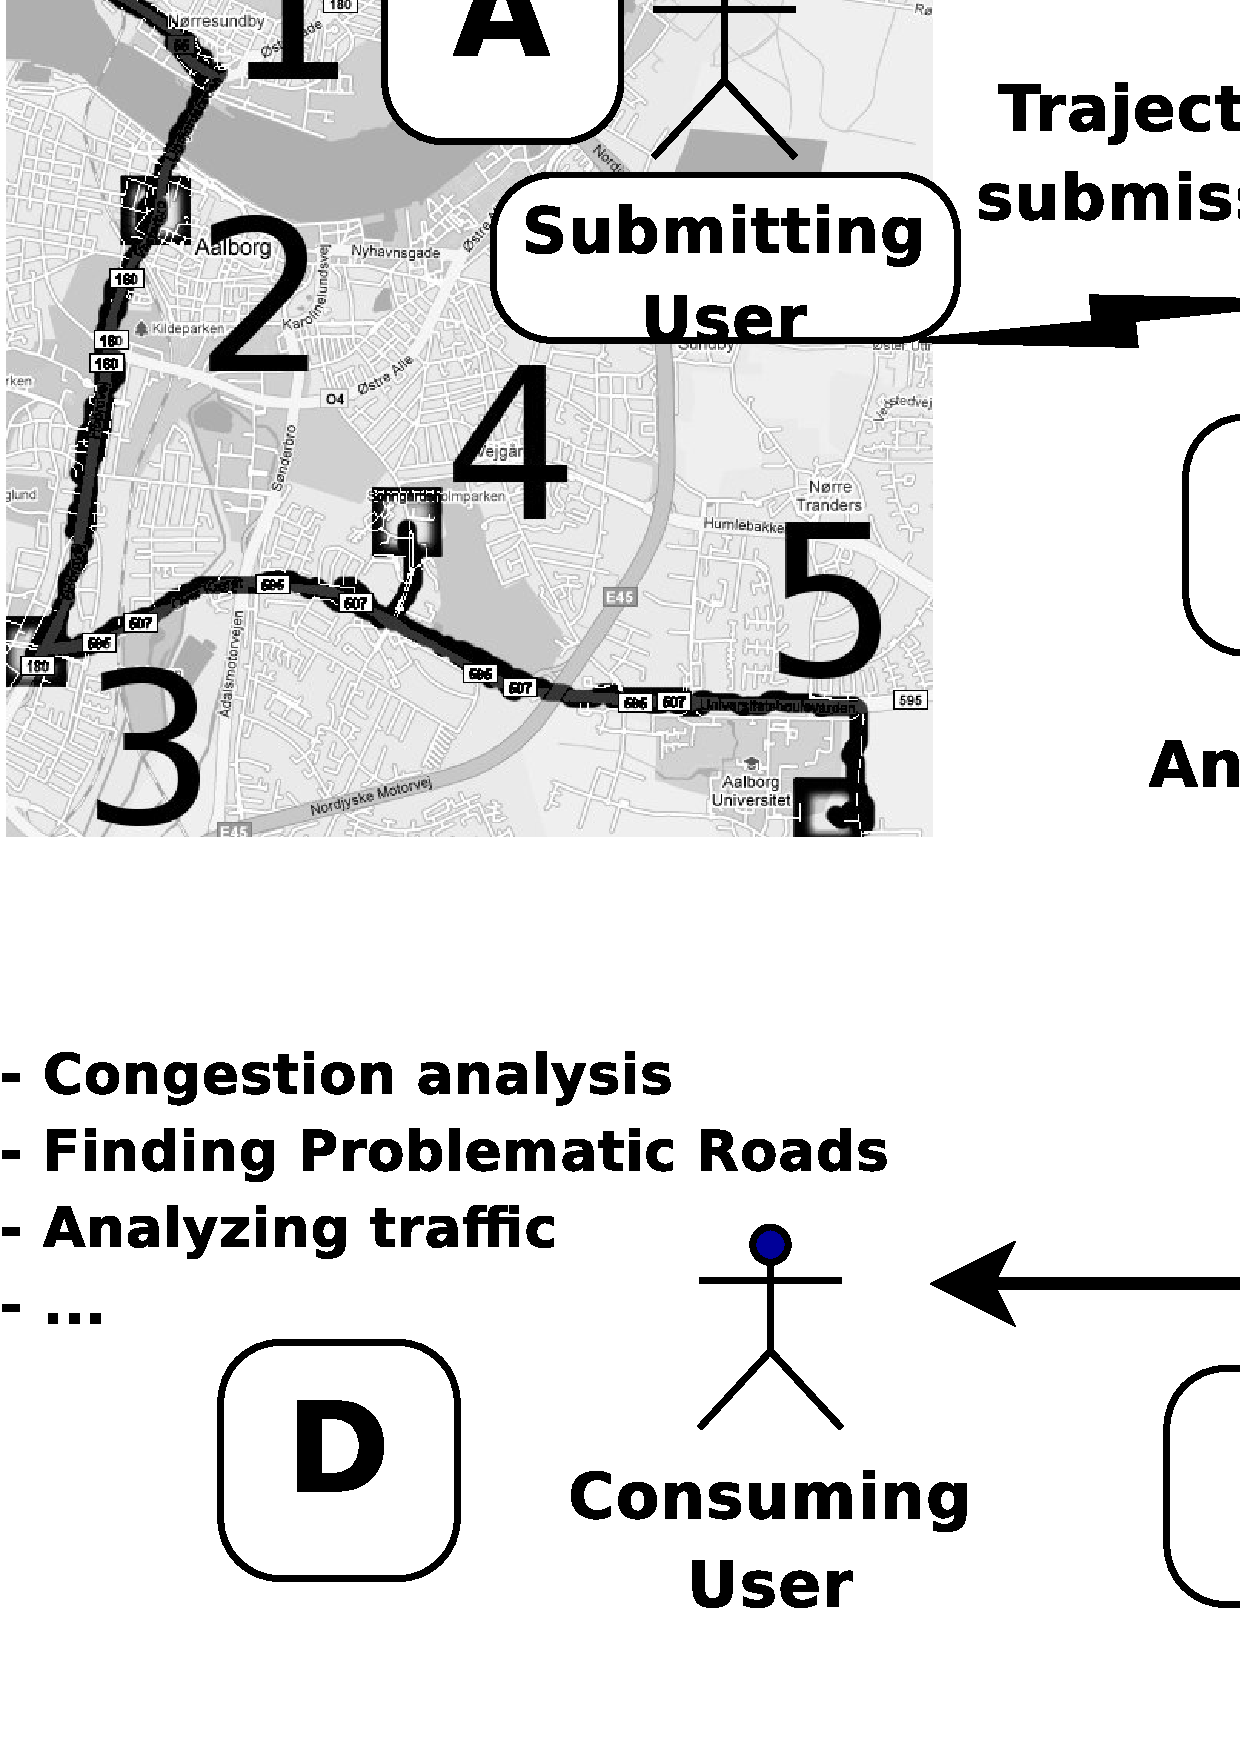
\includegraphics[page=1,scale=0.2]{images/overview.pdf}}
	\end{column}
	\begin{column}{0.5\textwidth}
		\begin{description}\itemsep 16pt
		\item[A] Privacy Aware User
		\item[B] Trusted Server
		\item[C] Public Untrusted Server
		\item[D] Service Providers
		\end{description}
	\end{column}
\end{columns}
\end{frame}%
\section{Baseline Competitors}

Intro to section; Why do we have baseline competitors, which ones will be introduced, and why those? 

LRU is a competitor, but can not achieve good performance because:
\begin{itemize}	
	\item Has no way to determine the usefulness of adding a path (i.e. no scoring function)
	\item Even if a path P is good (covers many queries), then if a sequence of consequtive queries comes which P can not cover, then it will be evicted.
	\item Has no way to optimize the number of paths in the cache, so available cache space may go unused.
	\item Querying the cache may require a scan of all paths in the cache
\end{itemize}

\section{Contribution} \label{sec:contribution}

Intro to section \\
Show benefits of a static cache over a dynamic cache.\\
List all advantages of a static cache solution \\
(\textit{Static cache} solves goal 2. has zero maintenance cost after filling the cache.)

explain what will be introduced, which sub-problems are considered, and which subsections presents what.


\subsection{Benefit model}
define benefit equations\\
Define optimization goal as a mathematical expfression to be minimized.

\subsection{Hardness Analysis}
Theoretical analysis showing how hard the problem is to solve for \spath caching.\\
show it is NP-Hard
 

\subsection{Greedy algorithm}
shows in more detail how we propose to solve our problem


\subsection{Statistics extration}

\subsubsection{Partition map} 
solves goal 1. reduce time on SP calc as it aids the cache with information on which paths may be useful.\\ 
discussion of kD-Tree.


\subsection{Cache representations and cache concepts} 

\subsubsection{Simple array of paths} - baseline for goal 2, unoptimized and expensive to use.

\subsubsection{Simple array of paths inverted list} - solves goal 2, reduces the query time of the cache.

\subsubsection{Graph representation} - solves goal 1, allows for more paths in cache, which should translate more cache hits.

\subsubsection{Sharing subpaths} - solves goal 1, allows for more paths in cache, translating to more cachehits. Unfortunally has a negative impact on goal 2 as it introduces some overhead in query time.

%
\section{Analysis}\label{sec:analysis}

Write theoretical analysis to show how hard the problem is to solve for \spath cacheing.
\section{Experiments}
We perform experiments using two different datasets and compare our method to two baseline approaches. Our approach \osc is compared to \lru and \fifo

\ffh{intro of section and what will be presented, and in which order}

\ffh{briefly mention the implementation}

\ffh{if possible find a baseline to compare with.}


\subsection{Data Generation}

We generate queries with random start-/end-nodes in two ways: completely random and Gaussian distribution.


\ffh{Use Brinkhoff to generate realistic start-/end-pairs based on where people actually want to go (give OSC an advantage). Explain the Brinkhoff data generator, the facts about the Oldenburg map and the generator parameters}

The test program has been implemented in C++ and the tests have been run on a Core2 Duo@2.8GHz with 4 GB memory. Timings has been measured using normal clock time, with mapdata preloaded into memory.


\subsection{Test Parameters}


\begin{tabular*}{\columnwidth}{|l | p{0.77\columnwidth}|}
\hline \textbf{Parameter} & \textbf{Purpose} \\\hline
numqueries & number of queries used \\\hline
cacheSize & Number of nodes which can fit in the cache \\\hline
gaussian & Whether to use Gaussian distribution when generating queries \\\hline
useNodeScore & use number of nodes in a cache element when calculating score in \osc \\\hline
useHitScore & use number of cache hits of a cache element when calculating score in \osc \\\hline
double sigma & sigma value when $gaussian$ is specified \\\hline
\end{tabular*}




\subsection{Experiments}

\ffh{Write some test, generate graphs of them, explain graphs}

\ffh{explain why we have chosen the tests we have}

% \section{Conclusion}
\subsection{Conclusion} % Bookmark information, displayed in the progress tree
\begin{frame}[red] %hmm.. thought i could change colour here :S
\frametitle{Conclusion}

\begin{itemize}
	\item Novel Privacy Profile to specify spatial-temporal sensitivity of a POI.
	\item Introduced t-anonymity
	\item Introduced Protection types and schemes.

\end{itemize}

 
\end{frame}

\subsection{Future Work} % Bookmark information, displayed in the progress tree
\begin{frame}[red] %hmm.. thought i could change colour here :S
\frametitle{Future Work}

\begin{itemize}
	\item Algorithm
	\item Performance study

\end{itemize}
\end{frame}


\begin{frame}[red] %hmm.. thought i could change colour here :S
\frametitle{End of Presentation}

\vspace{20mm}
\begin{center}
    \Huge Thank You For Listening
\end{center}

\end{frame}


%\newpage
%\section{HELP}




% 
% \section{Approach}
% 
% 
% \subsection{Specifying Sensitivity}

\section{what makes trajectories usable - usability}

\subsection{users}
They are good enough if the users privacy requirements are fulfilled

\subsection{data consumers}

If there is enough precision and data available such that the data consumers can make good services.







\begin{verbatim}
we rank spatial sensitivity:
0. none
1. low
2. medium
3. high

We rank temporal sensitivity:
0. none
1. low
2. medium
3. high


Identify type of POI 
(can be given by user):
1. Place/area (Hospital, Neighborhood, 
   city.)
2. Route w/o endpoints
3. Route w. endpoints
4. 


Start with all routes w. endpoints, 
then do all routes w/o endpoints and 
last do all area/place POI


case one:
Rank POI
\end{verbatim}














\begin{algorithm}[!Hbt]
    \dontprintsemicolon
    \SetVline

    \KwData{ 

  	$t \in \mathbf{T}$ - trajectory

	$u_p$ - a user profile

	$p \in \mathbf{P}$ - current POI

	
    }


%	\funcc{

    \funcc{poiTypeOne}{}
    {
	temporal \& spatial sensitivity
	}

	$g_l \leftarrow \{id(g) | g \in \Gamma(level): loc(u) \in g\}$ ;

	$\mathbf{g_v} \leftarrow \{id(g) | \forall g \in \Gamma(level): g
\cap vic(u) \neq \emptyset\}$;

	\textbf{return} ($g_l$, $\mathbf{g_v}$);
%    }
% 
    \funcc{poiTypeTwo}{}
    {
	$g_l \leftarrow \{id(g) | g \in \Gamma(level): loc(u) \in g\}$ ;

	$\mathbf{g_v} \leftarrow \{id(g) | \forall g \in \Gamma(level): g
\cap vic(u) \neq \emptyset\}$;

	\textbf{return} ($g_l$, $\mathbf{g_v}$);
    }
% 
    \funcc{poiTypeThree}{}
    {
	$g_l \leftarrow \{id(g) | g \in \Gamma(level): loc(u) \in g\}$ ;

	$\mathbf{g_v} \leftarrow \{id(g) | \forall g \in \Gamma(level): g
\cap vic(u) \neq \emptyset\}$;

	\textbf{return} ($g_l$, $\mathbf{g_v}$);
    }


    \funcc{onLocChange}{}
    {
        $wasPopped \leftarrow false$

        \While {$|GS| > 0$ \text{ and } $top(GS) \neq
mapLocToGranularity(|CS|-1)$}
        {
            Pop from stack $GS$;

            $wasPopped \leftarrow true$;
        }

        \If {$wasPopped$ \text{ or } $|GS| = 0$}
        {
            \textbf{pushAndSend}()
        }
    }

    \funcc{onMsgReceived}{M_{LevInc}, \text{Level } l}
    {
        \While{$|GS| \leq l$ \text{ and } $|GS| \leq L_{max}(u)$}
        {
            \textbf{pushAndSend}()
        }
     }

    \funcc{onMsgReceived}{M_{prox}, \text{Friend }  v, \text{Level} l}
    {
        Output "Friend ",$v$," with precision ", $L(l)$, " is inside
our vicinity!";
    }

\caption{The md's event handlers in our proximity based service.} 
\label{algCl}
\end{algorithm}

%\newpage
% \clearpage
%\section{Proposal of project parts}

% Mostly want to focus on the anonymization of GPS traces. I am having great difficulties coming up with a god way
% of doing this though. Not what I want the end result to be like, but more solution-wise how to archeve this in
% an efficient and nice way that I don't feel is just incremental compared to previous work.\\
% This is where I could use some suggestions on papers to read, keywords to think about, or maybe I could "just" take an
% existing suppression approach and use it with my concepts of time and sensitivity levels (see bullets below).
% 
% Remember I would like this to at some point be able to be published, so I want something that I can do alone, but
% I need help defining the scope of the project.
% I need your help on how to find the balance, so I can hopefully archeve this goal of a publication in the end of next
% this or next semester.
% (maybe suggestions on how to split the work, so I have a good project, but only "half" paper).\\

In the last meeting we talked about expanding, and classifying, the motivational scenarios, especially with regards to 
finding applications which has emphasis on working on subtrajectories. I have however been unable to come up with any good
scenarios, since I feel I am constantly ending up with more "density query" scenarios, which is not the kind of problem I want
to work on (which is why I have not added more scenarios in that category). 

Although I feel I have come a step closer to coming up with a solution for my proposed problem, my problem is still that I
feel like anything I come up with is too similar to existing work.

The "Preliminary Problem definition" more or less contains duplicate definitions for all concepts ("intro" \& subsections), this is on purpose, so I am
certain that I define all the concepts that I use so far. 

I am still a bit uncertain as to how much I should try to define in terms of classes/sets/tuples.



\subsection{Proposed system features}
\begin{itemize}
	\item Work on historical data (+ maybe updating the data continuesly with live data, depending on final solution).
	\item handle sensitivity groups for users with time (different groups sensitive at different times).
Groups are ways for "the system" classify users based on how much privacy they want in a given area, at a specific
time range. Privacy is here the degree of anonymization a user wants guarantied to be willing to publish his data.
	\item Have possibility to weight what is most sensitive factor when trying to anonymize: temporal or spacial.
Taking the two extremes: only using temporal or spacial anonymization, they have the following impact:
	\begin{itemize}
		\item Using the spacial dimension as the important factor in anonymization the location of the users will be generalized
uptil a factor satisfying the users privacy settings (street, block, part of city, etc.)
		\item When considering the temporal dimension as the important factor in anonymization, the user will have his trajectory
generalized over a time interval, making it impossible to identify when exactly the user traveled on the trajectory.

The user may not have a problem with someone figuring out where is was at a single point in time, 
but he may not want someone to find out that he is taking the same route at different times every day.
	\end{itemize}
\end{itemize}



\subsection{Preliminary Problem definition}

In this section we introduce relevant notations, define system requirements and specify
the behavior of the proposed service. 

We assume a setting where all users are equipped with a \ac{MD} able to communicate and report
the users position. All  \ac{MD}s are online and are continuesly reporting the users location at
predefined intervals. We use the terms {\it user, mobile device, and client} interchangeable and 
denote the set of \ac{MD}s by  $\mathbf{U} \subset \mathbb{N}$.

Let us assume a 2D scenario, where the movements of users in $\mathbf{U}$ are restricted to a road network 
$G(V,E)$. $V$ is the set of vertices, where each one represents either a street intersection or an important 
landmark. $E$ is the set of directed edges, where each one represents the smallest unit of road segment. All
users $u \in \mathbf{U}$ are mapped to edges in $e \in \mathbf{E}$.

All users specify at least one privacy profile. Each privacy profile specify the privacy settings for each road segment $e$
such that for each road segment $e_i \in \mathbf{E}$ that the user traverses, the system will generalize $e_i$ in 
the spatio-temporal domain



\subsubsection{Users}
Users are represented by a set $U$ where each user $u \in U$

\subsubsection{Road network}
The approach will assume all users $u \in U$, move on a road network which we define as a graph $G(V,E)$. $V$ is the set
of vertices, where each one represents either a street intersection or an important landmark. $E$ is the
set of directed edges, where each one represents the smallest unit of road segment. 

\subsubsection{Trajectories}
As the lowest level, a trajectory is a set of tubles $(time,longitude,latitude)$ ordered by the time attribute. 
However, as the approach we want to end up with is going to work on a road network, a 
higher level of abstraction is more appropriate. We define $T$ as the set of trajectories, where each trajectory 
consist of an id$(tid)$ and sequence of edges traversed $(tid, \langle e_0,\ldots,e_j \rangle)$, where $e_i \in E$,
the set of edges. I assume trajectories only move on the road network, and users users must traverse the entirety
of an edge. 

\subsubsection{Historical data}
The historical data consist of $T$, sorted by start/end time. This enables the approach to use
an appropriate time slice $(tid_g,\ldots,tid_h)$, where $tid_i \in T$, to do spatial anonymization, or work on all of $T$
to do temporal anonymization


\subsubsection{Privacy settings}
For the approach to use, for the user, satisfactory levels of anonymization, the user needs to be 
able to specify how $sensitive$ different areas(auto mapped to the edges $e \mid e \in E$ included in the area) are to the
user at different times in the day. Users will also be put into groups



\subsection{Taxonomy on Spatial-Temporal}
The proposed solution works on the spatio-temporal domain. 
Since a place/object can have different degrees of sensitivity associated with it at different 
times it is important to consider both the spatial and the temporal domain when trying to ensure 
the privacy of users in the solution.



\subsection{Privacy Profile}

Privacy profiles are a class of time constrained objects specifying a users road segment constrained
spacial sensitivity for discrete time intervals.


\subsubsection{list of things user would like to specify}

\begin{itemize}
	\item Sensitive places / road segments
	\begin{itemize}
		\item various degrees of sensitivity, some road segments/locations may
		be more sensitive than others e.g. a user may find it annoying if
		people knew he was shopping in some fancy store where things are expensive,
		but only annoying, while he may be really upset if someone found out he
		was seeing a psychiatrist. Thus the two have different levels of sensitivity. 
		\item different sensitivity degree as different points in time. e.g. 
		the free clinic is not a sensitive point on the trajectory at 8 am or 4 Pm when
		the user is driving too and from work (assuming of cause it is on the path), but any
		other time it would be a highly sensitive location/area.
	\end{itemize}
	\item Different profiles, e.g. a work profile, vacation profile
	\begin{itemize}
		\item profiles could be activated with a time limitation, he could have a choice of doing 
		it either automatically or manually.
	\end{itemize}
	\item Minimum privacy 
	\begin{itemize}
		\item can be specified globally for any trajectory, or for each level of sensitivity
		according to the area (road segments) the user is passing through.
	\end{itemize}
	\item 
\end{itemize}

\subsection{Motivational uses}
For the users publishing their data, 
they might want to access the trajectory dataset (possibly through a third party service provider on the data) to e.g. enable their 
GPS device to make better route planning depending on the time and place (some GPS devices already have the ability to use 
semi-live data to be better at suggesting routes to the user).

The user may also use the data through a service provider to e.g. find car pooling opportunities to an from work based
on what other users also takes the (close to) same route within a user specified time interval.

The users might also just get nothing in return for publishing their trajectories, but might help the government (or
similar organization) to better plan and build roads in the future. For some people the sense of "importance" may 
be motivational enough to make them publish their data.



\subsection{Scenarios}
\begin{itemize}
	\item {\bf Premise}
	\begin{itemize}
		\item {\bf User} Users are willing to publish their trajectories, if they are guarantied that no sensitive
or personally identifying information is contained or deduceable from the data set.
		\item {\bf Company} Companies wants to be able to query a public database with trajectories. They want the data
to be as correct, complete and detailed as possible
		\item {\bf service provider:} Collects, maintains and anonymizes a database of trajectories. Will make this dataset 
available to Companies.
	\end{itemize}
	\item {\bf Density queries}
	\begin{itemize}
		\item {\bf Scenario One} A company wants to monitor when, and where, certain road segments are congested in order to
{[optimize the duration of red/yellow/green at certain points in time, to make traffic flow better],
[Advise the city about future investments in roads and public transport],
[devise a system (for e.g. GPS devices) which is always able to predict the fastest route from point A to point B, irrespective of the actual length of the suggested route]}
and thus make some money.
		\item {\bf Scenario Two} A city or government could use collection of trajectories to analyze where people are going 
to and from at different time intervals during the day, or even during the calendar year. This could be usefull to gain an 
understanding of the general traffic patterns on their road network. This information could be usefull at several granularities 
to plan investments in new roads, how often existing roads should be serviced, or just to devise an automatic road congestion 
warning system
	\end{itemize}
	\item {\bf Outlier detection}
	\begin{itemize}
		\item {\bf Scenario Three} The police could do analysis of speed outliers on the dataset to see which road segments people are often driving to fast, 
and then set up speed controls on those road segments more often. They could also look at the opposite, people stopping, on major roads, 
where people would not normally have reason to stop, this could indicate traffic accidents, which could prompt more police presence on those roads
to make people drive nicer.
		\item {\bf Scenario Four} It could be usefull to do trajectory similarity analysis on many different levels. If is was possible
for e.g. city officials to specify two points (or spatial areas) A/B they could do some analysis on how people who go from A to B travel i.e.
what routes/trajectories they take to travel from A to B. It could also be examined if pattern changes over a day/week/month/year.
This kind of analysis could e.g. be used to calculate the inter-dependency between roads, which could be used to predict the increase in
load on other roads if one road is closed for some reason (e.g. maintenance, accident, or obstruction from some activity like a caneval or the like)
		%\item {\bf Scenario Five} stuff...
	\end{itemize}
	
\end{itemize}
%\section{Related work reference}

reference support for related work section.

\subsubsection{On effective presentation of graph patterns: a structural representative approach}
They develop an approach that combine two focuses when mining patterns in graphs. 1. they introduce a method to relax the tightness of the pattern subgraph pattern matching, so they can have high support for subgraphs which are very similar, but not exact. 2. as many mining approaches return allot (often very similar) patterns, they propose a method to collapse similar patterns so the user is presented with something that is easier to get an overview of and gain an understanding of the data. \cite{napa08}


% @inproceedings{napa08,
%  author = {Chen, Chen and Lin, Cindy Xide and Yan, Xifeng and Han, Jiawei},
%  title = {On effective presentation of graph patterns: a structural representative approach},
%  booktitle = {CIKM '08: Proceeding of the 17th ACM conference on Information and knowledge management},
%  year = {2008},
%  isbn = {978-1-59593-991-3},
%  pages = {299--308},
%  location = {Napa Valley, California, USA},
%  doi = {http://doi.acm.org/10.1145/1458082.1458124},
%  publisher = {ACM},
%  address = {New York, NY, USA},
%  }


\subsection{Cache Invalidation and Replacement Strategies for Location-Dependent Data in Mobile Environments}
They develop two cache replacement and invalidation techniques for mobile clients communicating with a LBS. They argue that in the setting of spatial data and LBS then it is important to consider more than just the access time when doing cache replacement. They look at the spatial area where an object in the cache is valid as well as the direction the user is moving. They do this besides calculating the probability that this object will be accessed again.

Assumes all POI objects are fixed size and no updates will be made. \cite{cirslddme}

% @article{cirslddme,
%  author = {Zheng, Baihua and Xu, Jianliang and Lee, Dik L.},
%  title = {Cache Invalidation and Replacement Strategies for Location-Dependent Data in Mobile Environments},
%  journal = {IEEE Trans. Comput.},
%  volume = {51},
%  number = {10},
%  year = {2002},
%  issn = {0018-9340},
%  pages = {1141--1153},
%  doi = {http://dx.doi.org/10.1109/TC.2002.1039841},
%  publisher = {IEEE Computer Society},
%  address = {Washington, DC, USA},
%  }




\subsection{Nearest-Neighbor Caching for Content-Match Applications}

\cite{nnccma}
% @inproceedings{nnccma,
%  author = {Pandey, Sandeep and Broder, Andrei and Chierichetti, Flavio and Josifovski, Vanja and Kumar, Ravi and Vassilvitskii, Sergei},
%  title = {Nearest-neighbor caching for content-match applications},
%  booktitle = {WWW '09: Proceedings of the 18th international conference on World wide web},
%  year = {2009},
%  isbn = {978-1-60558-487-4},
%  pages = {441--450},
%  location = {Madrid, Spain},
%  publisher = {ACM},
%  address = {New York, NY, USA},
%  }



\subsection{Caching Content-based Queries for Robust and Efficient Image Retrieval}

They study how to do caching with Content-based Image Retrieval, and they support range and kNN queries. They focus on how to do caching when many of the queries are similar, but not the same (e.g. picture cropped or color changes) without polluting the cache. Their approach works in metric space and they develop an approximate method to check if the result can be satisfied by the cache. They archive good results, getting few direct cache hits, but still satisfying many queries from similar queries in the cache.

\cite{ccqreir}

% @inproceedings{ccqreir,
%  author = {Falchi, Fabrizio and Lucchese, Claudio and Orlando, Salvatore and Perego, Raffaele and Rabitti, Fausto},
%  title = {Caching content-based queries for robust and efficient image retrieval},
%  booktitle = {EDBT '09: Proceedings of the 12th International Conference on Extending Database Technology},
%  year = {2009},
%  isbn = {978-1-60558-422-5},
%  pages = {780--790},
%  location = {Saint Petersburg, Russia},
%  publisher = {ACM},
%  address = {New York, NY, USA},
%  }



\subsection{Caching Complementary Space for Location-Based Services}
They develop the notion of Complementary Space(CS) to help better use a cache on a mobile client. CS is different levels for representing the objects on a map within MBRs. At the lowest level they just show the object, and as the levels go up they include more and more objects within MBRs, looking at the trade of in communication up/down link from a mobile client. They always have the entire world represented within the clients cache, at different levels, and offer no solution to how they will handle server updates to the map.

This is very similar to \cite{pcsqm}, although the approach does not formally depended on an R-tree, they still use one and offer no viable alternative, which lessens the difference even more. Their results are better than their competitors, including \cite{pcsqm}, though it seems that they stop their graphs just before \cite{pcsqm} beats them.

% @incollection {ccslbs,
%    author = {Lee, Ken and Lee, Wang-Chien and Zheng, Baihua and Xu, Jianliang},
%    affiliation = {Pennsylvania State University, University Park USA USA},
%    title = {Caching Complementary Space for Location-Based Services},
%    booktitle = {Advances in Database Technology - EDBT 2006},
%    series = {Lecture Notes in Computer Science},
%    editor = {Ioannidis, Yannis and Scholl, Marc and Schmidt, Joachim and Matthes, Florian and Hatzopoulos, Mike and Boehm, Klemens and Kemper, Alfons and Grust, Torsten and Boehm, Christian},
%    publisher = {Springer Berlin / Heidelberg},
%    isbn = {},
%    pages = {1020-1038},
%    volume = {3896},
%    year = {2006}
% }


\subsection{Proactive Caching for Spatial Queries in Mobile Environments}

They develop an approach which uses the index of an R-tree to add context to a cache of spatial object on a mobile client. They develop several communication and space saving techniques by representing less important parts of the R-tree in more compact ways, or just not storing the lower nodes/leaves of the tree. They also formally prove the asymptotic bounds of their algorithms.

\cite{pcsqm}
% @inproceedings{pcsqm,
%  author = {Hu, Haibo and Xu, Jianliang and Wong, Wing Sing and Zheng, Baihua and Lee, Dik Lun and Lee, Wang-Chien},
%  title = {Proactive Caching for Spatial Queries in Mobile Environments},
%  booktitle = {ICDE '05: Proceedings of the 21st International Conference on Data Engineering},
%  year = {2005},
%  isbn = {0-7695-2285-8},
%  pages = {403--414},
%  doi = {http://dx.doi.org/10.1109/ICDE.2005.113},
%  publisher = {IEEE Computer Society},
%  address = {Washington, DC, USA},
%  }


\subsection{Aggregate Aware Caching for Multi-dimensional Queries}

They develop a method to re-use items in a cache for a data werehouse. They take advantage of the levels of aggregation which exist in OLAP query results and come up with a way where they can get aggregated results using full or partial more detailed data from the cache. The use most of the paper on showing and proving that their algorithms have a good running time and admit them selfes that the approach is not very mature, though they still manage to get resonable results.
\cite{lncs2000}

%@inproceedings{lncs2000,
% author = {Deshpande, Prasad and Naughton, Jeffrey F.},
% title = {Aggregate Aware Caching for Multi-Dimensional Queries},
% booktitle = {Proceedings of the 7th International Conference on Extending Database Technology: Advances in Database Technology},
% series = {EDBT '00},
% year = {2000},
% isbn = {3-540-67227-3},
% pages = {167--182},
% numpages = {16},
% url = {http://portal.acm.org/citation.cfm?id=645339.650140},
% acmid = {650140},
% publisher = {Springer-Verlag},
% address = {London, UK},
%} 


\subsection{DynaMat: A Dynamic View Management System for Data Warehouses}

\textbf{abstract:} Pre-computation and materialization of views with aggregate functions is a common technique in Data Warehouses. Due to the complex structure of the warehouse and the different profiles of the users who submit queries, there is need for tools that will automate the selection and management of the materialized data. In this paper we present DynaMat, a system that dynamically materializes information at multiple levels of granularity in order to match the demand (workload) but also takes into account the maintenance restrictions for the warehouse, such as down time to update the views and space availability. DynaMat unifies the view selection and the view maintenance problems under a single framework using a novel ��goodness�� measure for the materialized views. DynaMat constantly monitors incoming queri and materializes the best set of views subject to the space constraints. During updates, DynaMat reconciles the current materialized view selection and refreshes the most beneficial subset of it within a given maintenance window. We compare DynaMat against a system that is given all queries in advance and the pre-computed optimal static view selection. The comparison is made based on a new metric, the Detailed Cost Savings Ratio introduced for quantifying the benefits of view materialization against incoming queries. These experiments show that DynaMat's dynamic view selection outperforms the optimal static view selection and thus, any sub-optimal static algorithm that has appeared in the literature.
\cite{dynamat99}

%@inproceedings{dynamat99,
%  author    = {Yannis Kotidis and
%               Nick Roussopoulos},
%  editor    = {Alex Delis and
%               Christos Faloutsos and
%               Shahram Ghandeharizadeh},
%  title     = {DynaMat: A Dynamic View Management System for Data Warehouses},
%  booktitle = {SIGMOD 1999, Proceedings ACM SIGMOD International Conference
%               on Management of Data, June 1-3, 1999, Philadelphia, Pennsylvania,
%               USA},
%  publisher = {ACM Press},
%  year      = {1999},
%  isbn      = {1-58113-084-8},
%  pages     = {371-382},
%  ee        = {http://doi.acm.org/10.1145/304182.304215, db/conf/sigmod/KotidisR99.html},
%  crossref  = {DBLP:conf/sigmod/99},
%  bibsource = {DBLP, http://dblp.uni-trier.de}
%}


\subsection{Cache-Oblivious Data Structures and Algorithms for Undirected Breadth-First Search and Shortest Paths}

\cite{codsa}
% @incollection {codsa,
%    author = {Brodal, Gerth Stølting and Fagerberg, Rolf and Meyer, Ulrich and Zeh, Norbert},
%    affiliation = {BRICS, Department of Computer Science, University of Aarhus, DK-8000 Århus C Denmark},
%    title = {Cache-Oblivious Data Structures and Algorithms for Undirected Breadth-First Search and Shortest Paths},
%    booktitle = {Algorithm Theory - SWAT 2004},
%    series = {Lecture Notes in Computer Science},
%    editor = {Hagerup, Torben and Katajainen, Jyrki},
%    publisher = {Springer Berlin / Heidelberg},
%    isbn = {},
%    pages = {480-492},
%    volume = {3111},
%    year = {2004}
% }


\subsection{Cached Shortest-Path Tree: An Approach to Reduce the Influence of Intra-Domain Routing Instability}

They assume a network setting and try to reduce the time and computational load it takes when network topology changes, as well as prevent any links from being unreachable if the topology changes often. The propose a cache with shortest-path trees, arguing that even if the topology changes often, then it is mostly between the same configurations (e.g. a computer/router is turned off/on) meaning that a cache with the most common seen configurations will be able to drastically reduce the amount of computation needed to recalculate routing tables.

\cite{csptri}
% @article{csptri,
% author="ZHANG,Shu and IIDA,Katsuyoshi and YAMAGUCHI,Suguru",
% title="Cached Shortest-Path Tree : An Approach to Reduce the Influence of Intra-Domain Routing Instability",
% journal="IEICE transactions on communications",
% ISSN="09168516",
% publisher="The Institute of Electronics, Information and Communication Engineers",
% year="2003-12-01",
% volume="86",
% number="12",
% pages="3590-3599",
% URL="http://ci.nii.ac.jp/naid/110003221599/en/",
% DOI="",
% }



\subsection{On Designing a Shortest-Path-Based Cache Replacement in a Transcoding Proxy}


\cite{spcrtp}
% @article {spcrtp,
%    author = {Hung, Hao-Ping and Chen, Ming-Syan},
%    affiliation = {National Taiwan University Graduate Institute of Communication Engineering Taipei Taiwan},
%    title = {On designing a shortest-path-based cache replacement in a transcoding proxy},
%    journal = {Multimedia Systems},
%    publisher = {Springer Berlin / Heidelberg},
%    issn = {0942-4962},
%    keyword = {Computer Science},
%    pages = {49-62},
%    volume = {15},
%    issue = {2},
%    year = {2009}
% }


\subsection{Optimizing Graph Algorithms for Improved Cache Performance}

\cite{ogaicp}

% @article{ogaicp,
%  author = {Park, Joon-Sang and Penner, Michael and Prasanna, Viktor K.},
%  title = {Optimizing Graph Algorithms for Improved Cache Performance},
%  journal = {IEEE Trans. Parallel Distrib. Syst.},
%  volume = {15},
%  number = {9},
%  year = {2004},
%  issn = {1045-9219},
%  pages = {769--782},
%  doi = {http://dx.doi.org/10.1109/TPDS.2004.44},
%  publisher = {IEEE Press},
%  address = {Piscataway, NJ, USA},
%  }





\bibliographystyle{abbrv}
\bibliography{bibliography}\label{bibliography}
% You must have a proper ".bib" file

% before submission Insert that ~.bbl file into
% the .tex source file and comment out
% the command \texttt{{\char'134}thebibliography}.

\end{document}
%\textcolor{red}{ }